\chapter{Related Work}
\label{chap:related_work}
This chapter provides an overview of the existing literature on art tracking with IoT and blockchains, highlighting previous research, methods, and findings related to the research question. Lastly, we also provide an overview of this field's state of the art.

\section{Artwork Conservation}
When it comes to preserving artworks, several factors play a role. This includes their exposition to human factors as well as environmental variations \cite{woodenartworkmonitoring}. More specifically factors that can hamper artwork integrity include humidity, temperature, light, pollutants, and microbiological organisms \cite{riskassessment}. Usually, temperature and humidity are the most sensitive parameters \cite{riskassessment}. The monitoring of such factors can be of significant importance when it comes to artwork preservation and health \cite{environmentmonitoring}. In addition to the conservation of artworks in museums or galleries, there is also the aspect of ensuring the safety of artwork during transportation. 

\section{Artwork Transportation}
Collections of artworks have been exhibited for generations. More often than not, artworks are showcased at different venues around the world. The dangers imposed on artwork during transportation have been thoroughly researched and led to the development of innovative packaging and other safety measures \cite{artintransit}. Today there exist a number of companies that specialize in the transportation of artwork \cite{kraftels, hasenkamp, weltifurrer} just to name a few. The advertised solution often involves shock-absorbing as well as climate-controlled packaging. Even though these packaging solutions have been properly tested, many of the reviewed companies rely on customer trust when it comes to their effectiveness in real-world applications. This presents an opportunity for monitoring systems leveraging the potential of emerging technologies to further improve the artwork transportation process.

\section{Artwork Monitoring Systems}
Technological advancements have made it possible to study the impacts of transportation on the integrity of artwork in more detail. Numerous studies have been conducted regarding this matter. One such study, utilized a small logging device to gather information on shock and vibrations generated during transportation \cite{shockvibrationtransit}. The study found that during the several dozen transportations monitored, there was significant shock and vibration suffered by the artwork, even though the latest packaging techniques and appropriate means of transportation were used. This demonstrates that continuous monitoring of these parameters can be useful when it comes to verifying the integrity of the artwork after transportation.

In this context, \cite{woodenartworkmonitoring} proposes a system that collects information about the artwork's environment and its safety conditions in real-time. This information can then be used to determine the quality of the conditions of artworks. The system uses a low-cost \gls{iot} node that is able to operate with very low power consumption and thus allows for the realization of pervasive monitoring systems. This proposed system demonstrates how any violations can be detected as they happen or have already happened. 

The study by \cite{pactart} goes one step further and proposes a proactive approach to potential violations. The so-called PACT-ART architecture employs advanced computing techniques like data mining and business process intelligence to predict the future state of the process. PACT-ART is then able to point out any possible violations and recommend actions to mitigate the foreseen misbehavior. \cite{riskmonitoring} expands on this and presents a system allowing for continuous risk assessment during storage, handling, transport, and exhibition.

\section{Artwork Management and Documentation}
Correct and secure information about artworks is one of the main concerns in the art world \cite{bcartmarket}. New technologies such as blockchain, have been proposed as promising solutions to increase the transparency, traceability, validity, and provenance of artworks \cite{cyberartmarket}. Especially smart contracts and \glspl{nft} have demonstrated the potential of blockchain technology to revolutionize the art world. 

\textcite{nftopportunities} has shown the benefits of \glspl{nft} protecting digital assets by proving their existence and ownership. \textcite{creativeindustry} has suggested the application of \glspl{nft} beyond digital art, proposing to physically tag an \gls{iot} device to an artwork or sculpture to transfer and track ownership. The \gls{iot} device is designed such that an attempt to tamper with the device will result in a blockchain record. This would potentially reduce intermediaries by providing a verifiable certificate that proves ownership, custodial history, and authenticity of a physical asset.

Platforms such as \textcite{artory}, \textcite{4art}, and \textcite{verisart} have already started to deploy blockchain and are offering a way to digitally register an artwork introducing transparency and authenticity to the artwork, its history, and provenance \cite{bcartmarket}.


\textcite{artchain}, for example, developed a blockchain-based trading system for artworks that uses \glspl{nft} to represent physical artworks. Introducing traceability, irreversibility, and transparency into the art market. 

\textcite{artory}, is a company employing these concepts to tokenize physical artworks to create a secure record of art pieces' provenance and ownership.


In this regard, \textcite{nftminter} has proposed an advanced \gls{nft} Minter for a blockchain-based artwork trading system. 

\textcite{artrentalblockchain} developed an artwork rental system based on blockchain technology to facilitate lending artwork collections.


\section{Supply Chain Management}
\gls{scm} is another area where \gls{iot} is being used to improve processes. Similar to monitoring the environment around an artwork, \gls{iot} is being used in \gls{scm} to monitor the product state in order to ensure the right quality \cite{iotsupplychains}. Another technology that is innovating \gls{scm} is the use of blockchain. The combination of these two technologies in industrial systems and supply chains has been a "hot trend" in recent years \cite{industryiot}. Blockchain presents an opportunity to build a trust basis with its unique characteristic of immutability. This can be used to improve documentation and traceability of physical assets as well as ensure the authenticity of the asset as well as collected data. The work that follows has already been established in this context.

\textcite{modum.io} present a solution to monitor relevant environmental data while transporting medical products. Upon delivery, the collected data is checked for compliance by a smart contract and then stored on the blockchain. There the data is immutable and verifiable by any party. The proposed system comprises backend, frontend, and \gls{iot} sensor devices. The architecture and components of the system are shown in Figure \ref{fig:modum.io}. In addition to the Ethereum blockchain network, modum.io uses a relational database to store raw temperature data and user credentials. The mobile clients download the temperature data via Bluetooth from the sensors and submit it to the server, which sends it to the \gls{sc} to evaluate the regulatory compliance and store the result \gls{on-chain}.

\begin{figure}[ht]
    \centering
    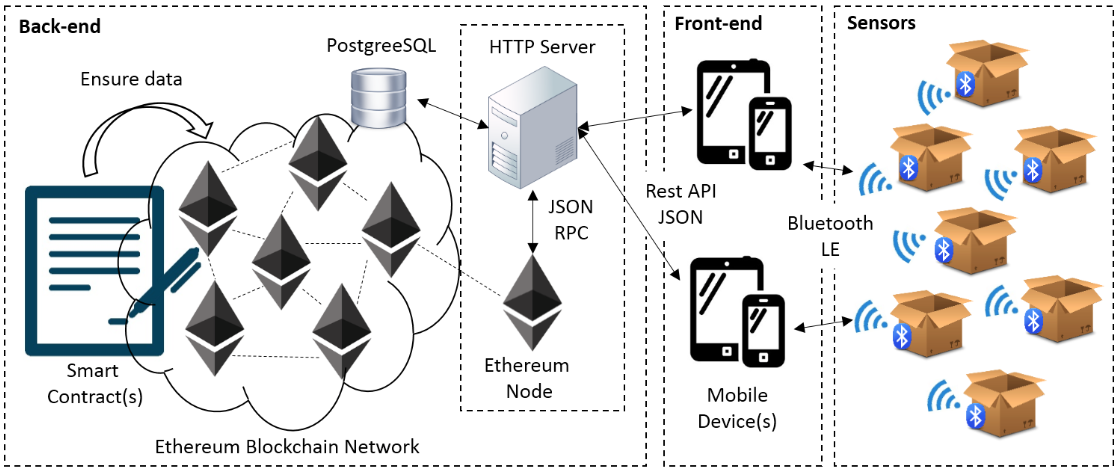
\includegraphics[width=0.8\textwidth]{diagrams/modum_architecutre.png}
    \caption{Modum.io AG Blockchain Architecture \cite{modum.io}}
    \label{fig:modum.io}
\end{figure}

\textcite{authena}, is a Swiss-based company that provides a platform for tracking and verifying the authenticity of physical assets using blockchain technology and \gls{iot}. Their platform offers three main products:
\begin{itemize}
    \item AUTHENA SHIELD: A tamper-proof end-to-end authenticity solution.
    \item AUTHENA L1VE: Real-time tracking of location and environmental conditions across countries and distribution channels.
    \item AUTHENA M3TA: Creating a secure link between physical product and its twin in the Metaverse.
\end{itemize}
According to \cite{authenahandelszeitung}, the system developed by authena is able to track the location as well as environmental data of an asset. This data is then stored securely and traceably on the blockchain. Unfortunately, the system is not open source and the company does not provide any technical insight regarding the architecture of the system.

\textcite{everledger}, is a digital transparency company providing technology solutions to increase transparency in global supply chains. They use blockchain to track and verify the authenticity of high-value assets such as diamonds, wine, and art. Their platform allows users to track the entire lifecycle of an asset, from production to ownership, using a secure and transparent blockchain-based ledger. Everledger mainly focuses on fraud detection, verification, and provenance records by issuing digital certificates stored on a private blockchain.

\section{Discussion}
% TODO: Discuss the 